\chapter{Presenting Your Venture}

Joseph Hadzima opens the evening as a two-part movement: first presenting the venture, then negotiating around it. Bob Jones takes the first part and, characteristically, does not begin with technique. He begins by justifying the subject. In a course built around practitioners, volunteers, and hard-won experience, presenting is not a cosmetic skill added after the business is understood. It is one of the places where we discover whether the business is understood at all. These notes follow that progression and keep the chapter anchored in the MIT OpenCourseWare lecture framed by Hadzima, delivered by Jones, and curated here by LazyingArt LLC.

\section{Why Presenting a Venture Belongs in the Course}

We begin where Jones begins: with a challenge. Why devote scarce course time to presenting a venture rather than to algorithms, market research, or some other more obviously technical subject? His answer is not abstract. A venture creates value only by persuading somebody to do something: buy, join, distribute, invest, stay, or eventually acquire. If we cannot describe the venture clearly enough to move one of those audiences, we have not merely failed at presentation; we have interrupted the mechanism by which the venture becomes real.

\subsection{Question \& Answer}

\paragraph{Question.} Why are we talking about presenting at all?

\paragraph{Answer.} Because presentation sits inside value creation. Jones walks the room through the obvious and the less obvious cases. We may need to acquire customers, recruit a channel partner, hire an engineer who has another offer, reassure a current staff after bad quarters, raise capital, or one day sell the company. Even family members may become an audience if the founder is about to reject a secure job and step into a startup with only a few months of cash. The lecture is therefore not about public speaking in the abstract. It is about the repeated act of aligning another person's action with the venture's next need.

That answer is strengthened by a second distinction. Jones reminds us that the entrepreneurial ladder has several rungs:
\begin{equation}
\text{Idea} \neq \text{Product}, \qquad \text{Product} \neq \text{Business}.
\end{equation}
A good idea still has to survive packaging, pricing, and execution. A good product still has to become a business. And a business, if it is understood, ought to be describable. Jones's test is merciless and useful: if someone asks about our company and, half an hour later, we are still searching for words, that is already evidence against our mastery of the business.

So the chapter cannot begin with stylistic advice. It must begin with the lecturer's deeper claim: the ability to describe the venture clearly and persuasively is itself one sign that the venture has taken coherent shape.

\section{Audiences, Objectives, and the Meaning of a Pitch}

Only after that motivational work does Jones narrow the frame. A pitch, he says in effect, is not just talk. It is talk with a goal.

\begin{definition}
A pitch is a presentation addressed to a particular audience \(A\), designed to produce some desired behavior \(Y\), organized around what that audience wants \(W_A\), and ending in the speaker's ask \(G\).
\end{definition}

We may compress his questions into a single formal line:
\begin{equation}
\text{Pitch}=(A,\ Y,\ W_A,\ G).
\end{equation}
That notation is editorial, not original to the slide deck, but it is faithful to Jones's own sequence: whom are we talking to, why are we talking to them, what do they want, how do we give them what they want, and what do we want from them?

At this point the lecture pivots from general communication to audience-specific design. The surviving slide frame is valuable precisely because it records that pivot in mid-reveal rather than after the full list is already visible.

\begin{figure}[h]
\centering

\includegraphics[width=\linewidth]{lecture_06_figure_02.png}
\caption{Partial audience slide as revealed in class: customers and potential employees. The frame records an intermediate state of the argument rather than the full later list.}
\end{figure}

The visible image supports only the first two items:
\begin{equation}
A_{\text{slide}}=\{\text{Customers},\ \text{Potential employees}\}.
\end{equation}
But Jones immediately extends the spoken list:
\begin{align}
A_{\text{full}} \approx \{\text{customers},\ \text{potential employees},\ \text{current employees},\ \text{channel partners / retailers},\ \text{family members},\ \text{investors}\}.
\end{align}

\begin{remark}
The image should not be over-read. It is evidence for the staged emergence of the audience taxonomy, not for the full taxonomy itself. The additional audiences come from the transcript, not from the frame.
\end{remark}

This staged reveal matters. Jones is not merely listing stakeholders. He is preparing the next question: if these audiences are different, do they really share the same priorities?

\subsection{Question \& Answer}

\paragraph{Question.} Should every audience hear the same pitch?

\paragraph{Answer.} No. Jones asks this directly and answers it directly. The investor, the recruit, the customer, and the nervous parent are not asking the same question, so they should not receive the same framing. The underlying venture may be the same, but the order of emphasis, the benefits highlighted, the evidence offered, and the final ask must change with the audience.

\section{The Audience's Hidden Question: WIFM}

Now the lecture makes its first real compression. Jones introduces the sales acronym WIFM:
\begin{equation}
\mathrm{WIFM}(A)=\text{``What's in it for me?''}
\end{equation}
The point is not merely salesmanship. The point is that every audience carries a payoff function into the room. They may be too polite or too sophisticated to ask the question aloud, but they are asking it internally, and a good pitch answers it before they have to do that work themselves.

For the customer, the translation is straightforward. The customer wants a problem solved. Jones's examples are ordinary on purpose: will this app get me where I want to go quickly and efficiently? will this suit help me look right in the board meeting? The question is always local and practical. The audience wants to know whether the venture gets them what they want.

For the recruit, the question changes. A new engineer may think the technology is interesting, but that is not top of mind. Can I pay my bills? Will this company survive long enough for my effort to matter? Am I joining a place where I can make a real difference, or just admire the founder's technology from the cheap seats? The recruit is still asking WIFM, but it is a different WIFM.

The pitch therefore has an internal order. Jones circles around it repeatedly, and we may write it in a cautious reconstructed form as
\begin{equation}
\text{Pitch order}(A)=B_A \to R_A \to G,
\end{equation}
where \(B_A\) is the benefit for audience \(A\), \(R_A\) is the reason to believe, and \(G\) is the ask. If we broaden that one step farther back, we get the fuller narrative chain:
\begin{equation}
\text{Problem} \to B_A \to R_A \to G.
\end{equation}

A compact diagram is useful here because the lecture itself is moving from audience taxonomy to a mechanism for tailoring the pitch:

\begin{figure}[h]
\centering
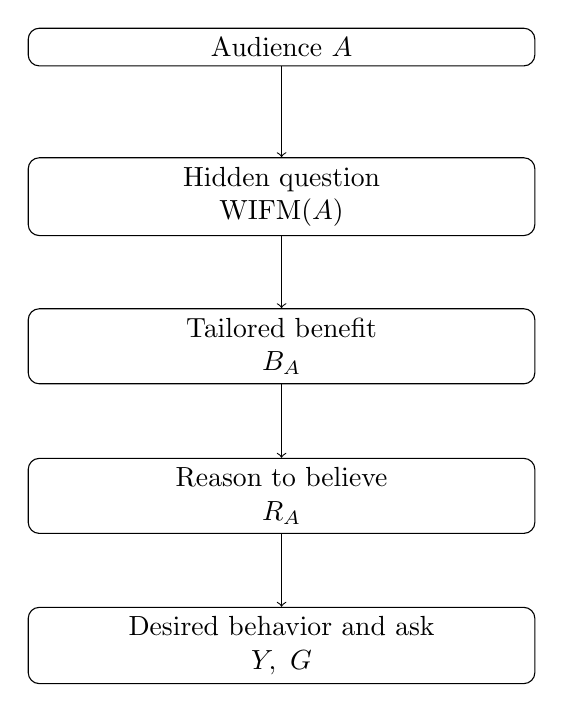
\begin{tikzpicture}
\node[draw, rounded corners, align=center, text width=6.2cm] (a) at (0,0) {Audience \(A\)};
\node[draw, rounded corners, align=center, text width=6.2cm] (b) at (0,-1.9) {Hidden question\\\(\mathrm{WIFM}(A)\)};
\node[draw, rounded corners, align=center, text width=6.2cm] (c) at (0,-3.8) {Tailored benefit\\\(B_A\)};
\node[draw, rounded corners, align=center, text width=6.2cm] (d) at (0,-5.7) {Reason to believe\\\(R_A\)};
\node[draw, rounded corners, align=center, text width=6.2cm] (e) at (0,-7.6) {Desired behavior and ask\\\(Y,\ G\)};
\draw[->] (a) -- (b);
\draw[->] (b) -- (c);
\draw[->] (c) -- (d);
\draw[->] (d) -- (e);
\end{tikzpicture}
\caption{Transcript-derived pitch logic in narrow form. Once the audience is fixed, the pitch must be translated through that audience's own WIFM.}
\end{figure}

This is the chapter's main invariant. Once we lose sight of it, the audience is forced to translate for us, and the pitch begins to fail.

\section{Baseline Pitches and What They Reveal}

Jones changes tempo by making the room do the work. He announces an ``equal opportunity embarrassment program'' and invites volunteers to pitch. That move matters pedagogically. He does not want the rule to arrive as a clean abstraction from nowhere. He wants the class to watch the rule emerge from failure, repair, and comparison.

The first volunteer, Andres, is building a venture around generative tools for video production. Once pressed to name the audience, he chooses prospective engineers. But his three-minute pitch is about hard computer-vision problems, market growth, and technical challenge. It is not nonsense. It is simply pointed at the wrong target. The class notices at once that they have heard almost nothing about the job itself. If we had to apply on the basis of the pitch alone, we would not know the role, the opportunity, the growth path, or even the practical reason to join.

Jones's repair is revealing. He keeps the unmet need in video editing, keeps the technology in the background as support, and pivots quickly to the recruit's benefit: come somewhere you can matter; come somewhere you are not one of 40,000 employees in a giant firm; come somewhere your skill changes the outcome. In other words, the repair works because the pitch is translated from technical description into audience-specific benefit.

The second volunteer, Subhash, brings an ultrasound venture and pitches to investors. This failure is different. Here the talk contains a real problem and a real technology, but the path from problem to business is muddy. The opening question about who likes hospitals wastes time. The user, the buyer, and the payer drift in and out of focus. The investor does not yet know who pays, how far along the venture is, whether traction exists, or why the solution is economically compelling. Again Jones intervenes, this time by giving a model pitch of his own. He starts from the burden placed on a specific high-risk patient group, moves through the inadequacy of ordinary telehealth, states the improved diagnostic capability, adds reimbursement as proof, and then arrives at the capital raise.

That is the diagnostic value of the exercise. A weak pitch is not merely ``bad.'' It usually reveals exactly where the entrepreneur has failed to connect audience, benefit, proof, and ask.

\subsection{Question \& Answer}

\paragraph{Question.} What went wrong when the pitch did not match the audience?

\paragraph{Answer.} In each case, the speaker made the listener perform the translation. The recruiting pitch never made the job legible to a recruit. The investor pitch made the investor wait too long for business logic. In both cases, the audience had to infer what the benefit was, who the relevant decision-maker was, and what action was being requested. Jones's critique is therefore less about eloquence than about structure.

\section{Benefits First, Then Reason to Believe}

Once the class has watched those failures, Jones becomes more explicit. The governing principle is simple and he states it more than once in different ways: benefits first, reason to believe second.

We can formalize the rule with the notation already in hand:
\begin{align}
B_A &= \text{the payoff the audience cares about},\\
R_A &= \text{the evidence that this payoff can actually be delivered}.
\end{align}
The novice entrepreneur often wants to start with \(R_A\): the algorithm, the patent, the founders, the brilliance of the vision, the claim to be ``visionary.'' Jones is not denying that such things matter. He is saying that they matter only if they give the listener a reason to believe the benefit.

This is why his reconstructed pitch order is
\begin{equation}
\text{Problem} \to B_A \to R_A \to G.
\end{equation}
The listener first needs to recognize a problem, then care about the benefit, then believe that we can deliver it, and only then entertain the ask.

His examples sharpen the point from several angles. The cell-phone example is deliberately stripped down. If we begin by describing marvelous technology, the audience still has to decide whether to care. If we begin with the benefit---your phone can be instantly recharged just when the battery is dying---interest arrives before mechanism. The mechanism then returns as support.

The same logic explains the lecture's long paraphrase of Leonardo da Vinci's letter. Jones does not present Leonardo as saying, ``Duke, observe how ingenious my engineering is.'' He presents him as saying, in effect, ``Here is what I can do for your war.'' Bridges, siege devices, armored wagons, ways to destroy the enemy's position: benefit after benefit, all in the Duke's language. The Duke does not need to love the technology first. He needs to want the outcome.

The Nordstrom story lands the same rule in ordinary commerce. The salesman asks what work Jones does, infers what kind of suit he needs, and supplies the version of Jones he wants to become. Only afterward do cloth quality and buttonholes appear as reason to believe. The sale happens because the benefit has already been internalized.

Jones also strengthens the rule with a story principle. When he later imagines ``Mabel'' dreading the hospital trip, he is not ornamenting the pitch. He is linearizing it. Story pulls the audience through the causal chain in the right order. It is much easier to say
\[
\text{Mabel's problem} \to \text{Mabel's burden} \to \text{better solution}
\]
than to dump disconnected facts about telehealth, imaging, insurance, and device architecture and hope the audience assembles them correctly.

He adds one further qualification. Believability matters. Conviction and enthusiasm help, but not to the point of lunacy. The entrepreneur who refuses all feedback, like the salsa seller who insists the product is perfect when the customer says it is too hot, is not demonstrating confidence. He is destroying the sale. Support must support; it cannot bulldoze.

\section{Delivery Under Constraints: Time, Memory, Voice, and Practice}

The lecture now moves from content to constraint. Jones is careful here. The right structure can still fail if it arrives too fast, too long, or physically inaudible. Presentation is therefore a bounded system. It has hard limits.

The first limit is memory:
\begin{align}
N_{\text{remembered}} &\approx 3,\\
N_{\text{sentences}} &= 3,\\
t_{\text{value prop}} &\approx 10\,\text{s}.
\end{align}
Most people, Jones says, will not remember more than about three things, and usually the three things most relevant to them. That observation yields his closing challenge: express the value proposition in three sentences and ten seconds. He calls it brutal, and it is. But it gives the venture a north star. On dark nights, when the founder is not sure what exactly is being built, the ability to say it in that compressed form becomes a test of understanding.

The second limit is attention:
\begin{equation}
t_{\text{attention loss}} \approx 30\,\text{s}.
\end{equation}
If the audience is bored or confused for much more than that, the phone comes out and we are done. Jones's advice here is not decorative. It is structural. If we have six minutes of material and only four minutes of time, we do not solve that by speaking faster. We solve it by editing.

His summary of brevity is comic and exact: be clear, be brief, and shut up.

The third limit is physical intelligibility. Jones tells a pitch-contest story in which he wins not because he had the most brilliant deck, but because he was the only speaker the judges could understand. That leads into the most practical technical instruction in the lecture:
\begin{equation}
d_{\text{mic}} \approx 2\text{--}4\,\text{in}.
\end{equation}
These microphones are directional. We speak down the barrel, not over the top, not off to the side, and not from six or eight inches away. If we like to point, we should point with the other hand. Otherwise excitement itself becomes noise.

Finally comes practice. Here Jones sounds almost musical, which fits his own background. To look easy, one usually has to work hard. He describes giving talks to empty rooms with a timer, cutting material when the clock exposed bad editing, even taping pictures to chairs so that eye contact itself could be rehearsed. These are not theatrical extras. They are part of building new habits. The founder used to talking about substance in technical language now has to talk about benefits, story, and pace. That retraining takes repetitions.

\section{Investor Logic and the Economics of Proof}

Only after the broader pitch framework is in place does Jones specialize to venture capital. This order is important. Investors are one audience among several, but they are an audience whose logic is unusually easy to compress.

Before the meeting itself comes access. The cold call is nearly dead on arrival:
\begin{equation}
N_{\text{cold calls/week}} \approx 200.
\end{equation}
Jones's point is not simply that venture capitalists are busy. It is that cold outreach has already failed the first filter. A warm introduction is better because it carries two hidden tests. First, is there fit? A software company may not belong in front of a healthcare-only investor. Second, will the introduction make the referrer look foolish? That is another form of WIFM. If the answer is yes, the introduction never happens.

\subsection{Question \& Answer}

\paragraph{Question.} What do investors actually want to know?

\paragraph{Answer.} Jones reduces the situation to two large questions:
\begin{align}
Q_{\text{inv}}^{(1)} &= \text{How will you make money?},\\
Q_{\text{inv}}^{(2)} &= \text{How will I make money?}
\end{align}
Everything else is subordinate. Under \(Q_{\text{inv}}^{(1)}\) sit the familiar business questions: what is broken, why is the solution better, are customers emerging, who is on the team, how will sales happen, what about manufacturing, what about IP? Under \(Q_{\text{inv}}^{(2)}\) sit terms, ownership, exit, and return.

Jones is also careful about what an initial investor pitch is for. It is usually not for finishing diligence. It is for winning the next question, the next meeting, the next layer of attention.

The lecture immediately tests that logic on a live case. Rita pitches an investor-facing software-recommendation venture. Her initial move is to ask the room several show-of-hands questions about AI adoption and discovery. Jones's reaction is brutal and useful: this is a colossal waste of time. The first 45 seconds of an investor pitch are too expensive to spend on generic audience participation, especially when the speaker is already holding stronger proof. What had been buried near the end turns out to be the true opening: she knows the market, has roughly half a million followers in that space, and has already made about \$80{,}000 in revenue. For investors, those facts are compressed forms of \(R_A\). They say, ``I know this market, I have access, and I am already seeing signal.'' Jones's rewritten opening therefore moves traction and credibility forward.

The lecture then returns to the ultrasound founder for a second try. This time the opening is linear and much stronger. He starts with headline market context, narrows to the high-risk segment, states the home-scan solution, and then names distinct benefits for doctors, hospitals, and insurers. Jones stops him early because the structure is already much better. The arithmetic in the classroom exchange is rough, but the order is right. The audience now sees the user, the problem, the solution, and the stakeholder-specific value in sequence.

\paragraph{Worked example.} Jones's clearest piece of economic reasoning comes from his own catheter-lab story. The structure is worth preserving carefully because it separates user enthusiasm from payer logic.

The facts unfold in stages:
\begin{enumerate}
\item Doctors want the device because procedures go better.
\item Patients benefit because surgery is shorter and recovery is quicker.
\item But neither doctors nor patients pay for adoption.
\item The actual economic decision-maker is the hospital purchasing function.
\item The cath lab makes money in proportion to the number of procedures performed.
\item Turnover lag between procedures is therefore economically important.
\item The device reduces that lag enough to add one more procedure per day.
\end{enumerate}
Jones summarizes the result numerically as
\begin{align}
\Delta n_{\text{procedures/day}} &= 1,\\
T_{\text{payback}} &\approx 6\,\text{weeks}.
\end{align}
He does not present line-by-line arithmetic, and we should not manufacture it. But the logic is clean. ``Doctors like it'' is not proof of value. ``The hospital earns one additional procedure per day and the device pays for itself in six weeks'' is proof of value. That is exactly the kind of translation from benefit to payer-specific evidence that the lecture has been building toward from the beginning.

\subsection{Question \& Answer}

\paragraph{Question.} Who should give the pitch?

\paragraph{Answer.} Jones answers with a distinction. Sometimes a team presentation is best. A chief technology officer may explain the technical side better than the CEO, and a chief marketing officer may explain go-to-market better than either. But he also says he has never seen an investor commit without confidence that the CEO can drive the bus. So the pitch may be distributed, but the founder is not exempt from it.

\section{Summary}

By the end of the lecture the method has been compressed almost to axioms. A pitch is not generic speech but a structured object:
\[
\text{Pitch}=(A,\ Y,\ W_A,\ G).
\]
The audience comes first. Every audience asks some version of WIFM. Therefore we do not begin with ourselves, our brilliance, or our technology. We begin with a problem, state the benefit in the listener's language, provide reason to believe, and then make the ask.

The later sections add the constraints that make the method operational. The audience remembers only a few things. Time cannot be cheated by speaking faster. Physical intelligibility matters. Practice is part of the construction of the pitch, not an afterthought.

Jones finally compresses all of this into a closing rule we can carry forward: know the audience, know the three things we want them to remember, show that we understand their problem, tell the story of the better solution, and practice until the delivery is economical and clear. In a venture course, that is not mere rhetoric. It is part of the venture's mechanism for becoming a business.